\documentclass[25pt, a0paper, portrait]{tikzposter}
\geometry{paperwidth=34in,paperheight=36in}

\title{Simulating Missile Trajectory with IVODEs}
\author{Colin Tierney}
\date{\today}
\institute{Modeling and Simulation Final}
\usebackgroundstyle{Default}

\usepackage{blindtext}
\usepackage{comment}

\usetheme{Default}
\definebackgroundstyle{Default}{
\draw[inner sep=0pt, line width=0pt, color=white, fill=white]
(bottomleft) rectangle (topright);}

\begin{document}

\maketitle
\node[anchor=west, xshift=-2cm] at (TP@title.west) {
\includegraphics[width=10cm]{images/mc-logo}};
\node[anchor=east, xshift=1cm, yshift=-.25cm] at (TP@title.east) {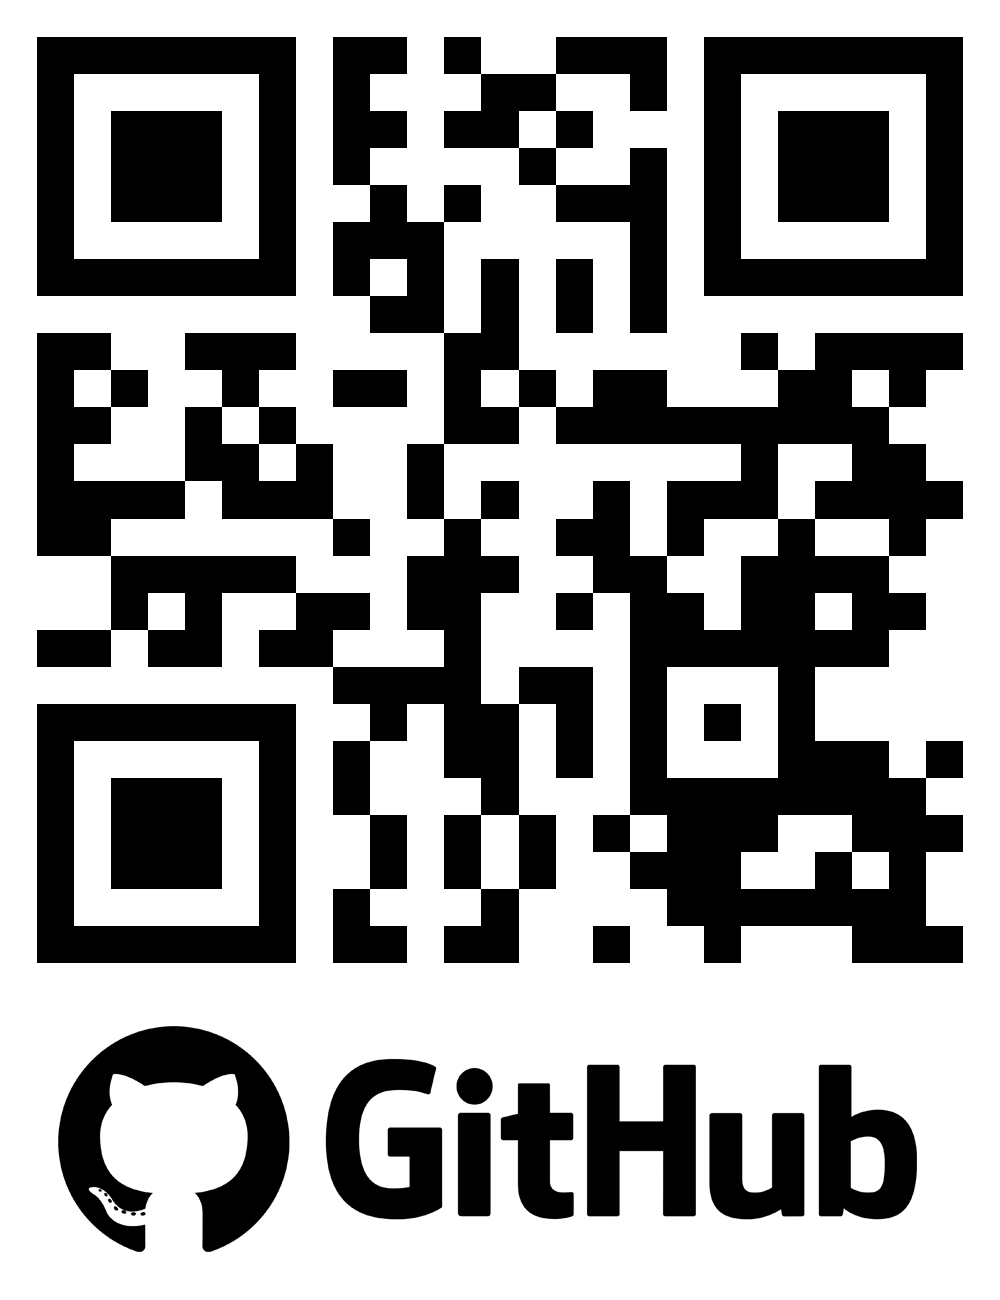
\includegraphics[width=8cm]{images/qrcode}};

\block{Introduction}
{
    In a ballistic missile trajectory simulation, the system of differential equations used to 
    describe the ballistic model is a highly complex system. In particular, the six-degree of 
    freedom model used most frequently, consists of a system of twenty-one 2nd order ordinary 
    differential equations, which are to be solved for the ballistic missile's components of 
    acceleration, velocity, and position at discrete time intervals. The usual method for 
    simulating missile trajectory is the 4th Order Runge Kutta method (commonly called RK4), which 
    is used to approximate a Taylor Series method that needs an initial condition of time and the 
    function itself to be given.  A newer algorithm, called the Parker-Sochacki Method (PSM for 
    short), which uses the Power Series instead of the Taylor Series, is what this report is going 
    to be diving into, as there are certain advantages compared to the RK4 system that is typically 
    used in most applications today.
}

\begin{columns}
    \column{0.4}
    \block{Assumptions}
    {
        
    }
    
    \column{0.6}
    \block{Problem Identification}
    {
        Here, \blindtext \vspace{4cm}
    }
    \note
    [
        targetoffsetx=-9cm, 
        targetoffsety=-6.5cm, 
        width=0.5\linewidth
    ]
    {e-mail \texttt{welcome@overleaf.com}}
\end{columns}

\begin{columns}
    \column{0.5}
    \block{Model Verification}
    {
        \begin{tikzfigure}
            
\includegraphics[width=0.2\textwidth]{images/overleaf-logo}
        \end{tikzfigure}
        \vspace{4cm}
    }
    \column{0.5}
    \block{Figures}
    {
        \blindtext
    }
    \block{Conclusion}
    {
        conclusion stuff
    }
\end{columns}
\block{References}
{
    \blindtext
}


\end{document}